%\documentclass[10pt]{beamer}
\documentclass[xcolor={pdftex,dvipsnames,table}]{beamer}

\definecolor{redUnipd}{HTML}{9b0014}
\definecolor{grayUnipd}{HTML}{444F51}
\definecolor{myblue}{HTML}{317a9b}
%\definecolor{Black}{RGB}{0,62,114}
\newcommand{\bbf}[1]{\textcolor{black}{\bf #1}}
\newcommand{\rbf}[1]{\textcolor{redUnipd}{ #1}}
\usefonttheme{structurebold}
\usecolortheme[named=myblue]{structure}
\setbeamercolor{structure}{fg=redUnipd}
\setbeamercolor{normal text}{bg=white,fg=grayUnipd}
\setbeamertemplate{itemize items}{$\circ$}
%\textopenbullet
%\usepackage{marvosym}
%\setbeamertemplate{itemize items}{$\Neutral$}

\usepackage{pgfpages}
\pgfpagesuselayout{resize to}[a4paper, 
                                border shrink=1.5cm,
                                landscape]


\usepackage[T1]{fontenc}
%
\usepackage[english]{babel}
\usepackage{graphicx}
\usepackage{booktabs}
\usepackage{latexsym}
\usepackage{subfigure}
\usefonttheme{professionalfonts}
%\usepackage{enumitem}
\usepackage{amsmath,amssymb}
\usepackage[latin1]{inputenc}
%\setbeamercovered{dynamic}
\usepackage{Sweave}
\usepackage[english]{babel}
\usepackage{tikz,comment,amssymb}
\usetikzlibrary{shapes}

\newcommand{\bb}[1]{\begin{block}{#1}}
\newcommand{\eb}{\end{block}}
\newcommand{\bi}{\begin {itemize}}
\newcommand{\ei}{\end{itemize}}
\newcommand{\be}{\begin {enumerate}}
\newcommand{\ee}{\end{enumerate}}
\linespread{1.05}

\newcommand{\bfr}[1]{\begin{frame} \frametitle{#1}}

\AtBeginSection[] {
  \begin{frame}<beamer>
    \frametitle{Outline}
    \tableofcontents[currentsection]
  \end{frame}
}


\title[]{Multiplicity Control in Clinical Trial}
\subtitle{False Discovery Rate}
\author[\hspace{5cm}]{Livio Finos}
\date{}% \date{A.A. 2015/2016 }
%\logo{
\includegraphics[scale=.05]{figures/logoUnipd.jpg}}

\begin{document}

\begin{frame}
  \titlepage
\end{frame}
% Goeman, A Solari

%%%%%%%%%%%%%%%%%%%%%
\begin{frame}
I thank Aldo Solari, Jelle Goeman and Florian Klinglmueller for the ideas and the materials we shared along these years. The material is the result of all this resoning together.

\end{frame}

\section{False Discovery Rate (FDR)}
\subsection{Definition}

% \begin{center}
% \begin{tabular}{ l | c c | r }
%                 & \# Non Rifiutate & \# Rifiutate  & Totale\\
% \hline
%   \# $H_0$ & $A_0$ & \rbf{$R_0$} & $m_0$\\
%   \# $H_1$ & $A_1$ & $R_1$ & $m_1$ \\
% \hline
%     & $A$ & \rbf{$R$} & $m$\\
% \end{tabular}
% \end{center}
% \bigskip
% 
% Controllare il \bbf{False Discovery Rate (FDR)}\\ significa definire una procedura che controlli il valore atteso del rapporto dei falsi rifiuti:\\
% $$E( \frac{\#  Falsi\ Rifiuti}{\# Rifiuti} ) =E(\rbf{\frac{R_0}{R}} ) \leq q$$ 
% \bigskip
% solitamente $q=.05$ (analogo $\alpha$)
% \end{frame}

\bfr{A contingency table}
\begin{table}[!ht]
  \bb{Contingency table for multiple hypothesis testing}
    Rejection versus truth or falsehood of hypotheses
    \newline\ \\
    \begin{tabular}{lccc}
                  & true    & false   & total \\\hline
    rejected      & $V$     & $U$     & $R$ \\
    not rejected  & $m_0-V$ & $m_1-U$ & $m-R$ \\\hline
    total         & $m_0$   & $m_1$   & $m$
    \end{tabular}
  \eb
\end{table}
\end{frame}


\bfr{FDP, FWER and FDR}
  \bb{False Discovery Proportion}
\[
\mathrm{FDP} = \left\{ \begin{array}{ll} V/R & \textrm{if $R > 0$} \\ 0 & \textrm{otherwise}, \end{array} \right.
\]
    Defined for every rejected set $R$
  \eb
  \bb{Familywise error rate}
   \[ \mathrm{FWER} = \mathrm{P}(V > 0) \]
  \eb
  \bb{False discovery rate}
    \[ \mathrm{FDR} = \mathrm{E}(\mathrm{FDP}) \]
  \eb
\end{frame}

\subsection{Methods}

\bfr{False Discovery Rate
\footnote{Benjamini and Hochberg (1995). Journal of the Royal Statistical Society, Series B (Methodological) 57 (1): 289--300.}}


% \section{Basic FDR  methods}
% \subsection{}
 \bb{BH procedure}
    \be
      \item Sort the $p$-values: $p_{(1)}, \ldots, p_{(m)}$
      \item Find $j'$, the largest $j$ such that $p_{(j)} \leq j\alpha/m$
      \item Reject all hypotheses with $p$-values at most $p_{j'}$
    \ee
  \eb
  \bb{Benjamini and Hochberg}
    This procedure controls FDR under independence
    \\ Control is at $\pi_0\alpha$ (compare Bonferroni), with $\pi_0=m_0/m$
  \eb
  \bb{Later}
    Conditions relaxed
  \eb
\end{frame}

\bfr{Step-down and step-up}
  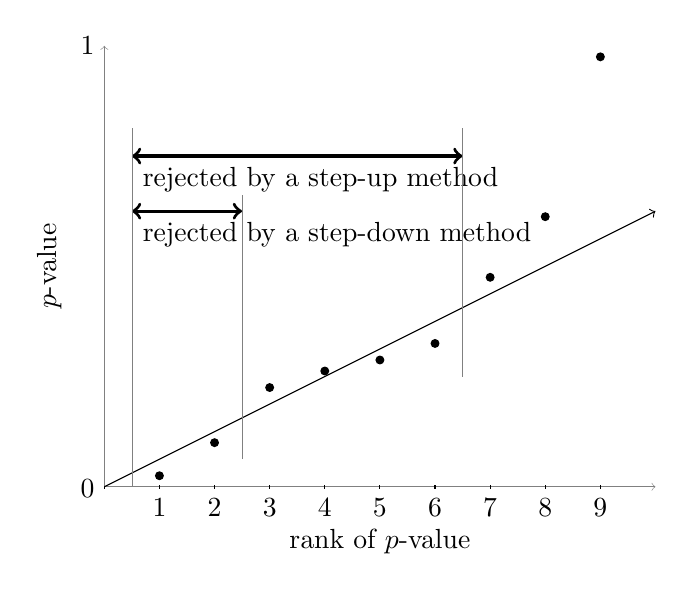
\begin{tikzpicture}[scale=.7]
    \draw[help lines, ->] (0,0)--(10,0);
    \draw[help lines, ->] (0,0)--(0,8) ;
    \path(0,8) node[left] {1};
    \draw[->] (0,0) -- (10,5);
    \draw[fill] (1,0.2) circle(2pt);
    \draw[fill] (2,0.8) circle(2pt);
    \draw[fill] (3,1.8) circle(2pt);
    \draw[fill] (4,2.1) circle(2pt);
    \draw[fill] (5,2.3) circle(2pt);
    \draw[fill] (6,2.6) circle(2pt);
    \draw[fill] (7,3.8) circle(2pt);
    \draw[fill] (8,4.9) circle(2pt);
    \draw[fill] (9,7.8) circle(2pt);
    \draw[<->, very thick, below right] (.5,6) node{rejected by a step-up method} -- (6.5,6);
    \draw[<->, very thick, below right] (.5,5) node{rejected by a step-down method} -- (2.5,5);
    \draw[help lines] (6.5, 2) -- (6.5,6.5);
    \draw[help lines] (2.5, 0.5) -- (2.5,5.3);
    \draw[help lines] (.5, 0) -- (0.5,6.5);
    \foreach \x in {1,2,3,4,5,6,7,8,9}
      \draw (\x, -1pt) node[below] {\x} -- (\x, 1pt);
    \draw (0,-1pt) node[left] {0} -- (0,0);
    \path (5,-1) node{rank of $p$-value};
    \path (-1,4) node[rotate=90]{$p$-value};
  \end{tikzpicture}
\end{frame}


\bfr{Benjamini and Hochberg (BH)}
\begin{overprint}
\onslide<1>  $\frac{p_{(10)} \ m}{10}=\frac{0.753 \ 10}{10} =0.753 \bbf{\stackrel{?}{\leq}  q=.10}$ : No
\onslide<2>  $\frac{p_{(9)} \ m}{9}=\frac{0.731 \ 10}{9} =0.812 \bbf{\stackrel{?}{\leq}  q=.10}$ : No
\onslide<3>  $\frac{p_{(8)} \ m}{8}=\frac{0.503 \ 10}{8} =0.629 \bbf{\stackrel{?}{\leq}  q=.10}$ : No
\onslide<4>  $\frac{p_{(7)} \ m}{7}=\frac{0.314 \ 10}{7} =0.449\bbf{\stackrel{?}{\leq}  q=.10}$ : No
\onslide<5>  $\frac{p_{(6)} \ m}{6}=\frac{0.153 \ 10}{6} =0.255 \bbf{\stackrel{?}{\leq}  q=.10}$ : No
\onslide<6>   etc. 
\onslide<7>  $\frac{p_{(2)}\ m}{2}=\frac{0.016 \ 10}{2} =0.080\bbf{\stackrel{?}{\leq}  q=.10}$ : Yes!, \textcolor{redUnipd}{STOP}
\end{overprint}


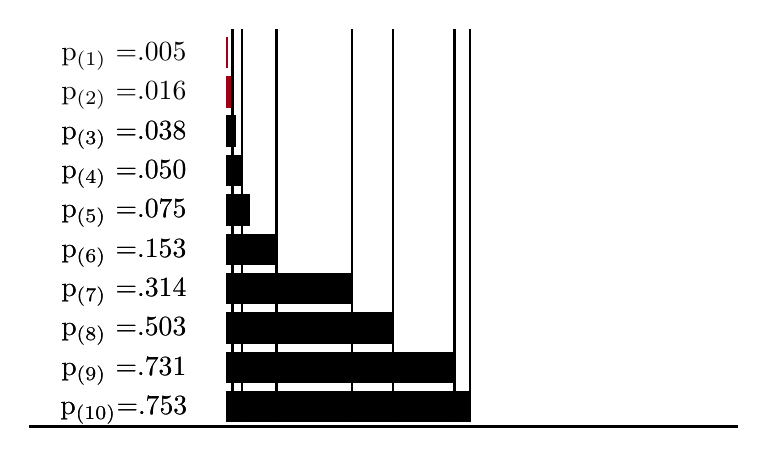
\begin{tikzpicture}

\draw<1>[thick] (5.6cm,0pt) -- (5.6cm,5cm);
\draw<2>[thick] (5.4cm,0pt) -- (5.4cm,5cm);
\draw<3>[thick] (4.62cm,0pt) -- (4.62cm,5cm);
\draw<4>[thick] (4.1cm,0pt) -- (4.1cm,5cm);
\draw<5>[thick] (3.14cm,0pt) -- (3.14cm,5cm);
\draw<6>[thick] (2.7cm,0pt) -- (2.7cm,5cm);
\draw<7>[thick] (2.58cm,0pt) -- (2.58cm,5cm);

\draw[very thick] (0cm,-.05cm) -- (9cm,-.05cm);

\fill<1>[redUnipd,xshift=2.5cm]           (0,0) rectangle (3.1cm,.4cm);
\node at (1.2,.15) {p$_{(10)}$=.753};
\fill<2->[xshift=2.5cm]           (0,0) rectangle (3.1cm,.4cm);
\node at (1.2,.15) {p$_{(10)}$=.753};
     
\fill<1-2>[redUnipd,yshift=.5cm,xshift=2.5cm] (0,0) rectangle (2.9cm,.4cm);
\node at (1.2,.65) {p$_{(9)}$ =.731};
\fill<3->[yshift=.5cm,xshift=2.5cm] (0,0) rectangle (2.9cm,.4cm);
\node at (1.2,.65) {p$_{(9)}$ =.731};

\fill<1-3>[redUnipd,yshift=1cm,xshift=2.5cm] (0,0) rectangle (2.12cm,.4cm);
\node at (1.2,1.15) {p$_{(8)}$ =.503};
\fill<4->[yshift=1cm,xshift=2.5cm] (0,0) rectangle (2.12cm,.4cm);
\node at (1.2,1.15) {p$_{(8)}$ =.503};

\fill<1-4>[redUnipd,yshift=1.5cm,xshift=2.5cm] (0,0) rectangle (1.6cm,.4cm);
\node at (1.2,1.65) {p$_{(7)}$ =.314};
\fill<5->[yshift=1.5cm,xshift=2.5cm] (0,0) rectangle (1.6cm,.4cm);
\node at (1.2,1.65) {p$_{(7)}$ =.314};

\fill<1-5>[redUnipd,yshift=2cm,xshift=2.5cm] (0,0) rectangle (.64cm,.4cm);
\node at (1.2,2.15) {p$_{(6)}$ =.153};
\fill<6->[yshift=2cm,xshift=2.5cm] (0,0) rectangle (.64cm,.4cm);
\node at (1.2,2.15) {p$_{(6)}$ =.153};

\fill<1-5>[redUnipd,yshift=2.5cm,xshift=2.5cm] (0,0) rectangle (.3,.4);
\node at (1.2,2.65) {p$_{(5)}$ =.075};
\fill<6->[yshift=2.5cm,xshift=2.5cm] (0,0) rectangle (.3,.4);
\node at (1.2,2.65) {p$_{(5)}$ =.075};

\fill<1-6>[redUnipd,yshift=3cm,xshift=2.5cm] (0,0) rectangle (.2,.4);
\node at (1.2,3.15) {p$_{(4)}$ =.050};
\fill<7->[yshift=3cm,xshift=2.5cm] (0,0) rectangle (.2,.4);
\node at (1.2,3.15) {p$_{(4)}$ =.050};

\fill<1-6>[redUnipd,yshift=3.5cm,xshift=2.5cm] (0,0) rectangle (.121cm,.4cm);
\node at (1.2,3.65) {p$_{(3)}$ =.038};
\fill<7->[yshift=3.5cm,xshift=2.5cm] (0,0) rectangle (.121cm,.4cm);
\node at (1.2,3.65) {p$_{(3)}$ =.038};

\fill[redUnipd,yshift=4cm,xshift=2.5cm](0,0) rectangle (.066cm,.4cm);
\node at (1.2,4.15) {p$_{(2)}$ =.016};

\fill[redUnipd,yshift=4.5cm,xshift=2.5cm] (0,0) rectangle (.02cm,.4cm);
\node at (1.2,4.65) {p$_{(1)}$ =.005};
\end{tikzpicture}
\end{frame}


\bfr{Meaning of FDR control}
  \bb{FDR control}
    On average, the $\mathcal{R}$ returned by BH has FDP $\leq\pi_0\alpha$
  \eb
  \bb{Variability of FDP}
    Due to variability of $\mathcal{R}$
  \eb
  \bb{Realized FDP}
    Varies around $\pi_0\alpha$.
    \\ Variability can be high if $p$-values correlated
  \eb
\end{frame}




\bfr{Benjamini \&\ Yekutieli (BY)\footnote{Benjamini Y, Yekutieli D. (2001) The control of the false discovery rate in multiple testing under dependency. {\it Annals of statistics} 29(4):1165--1188}}
  \bb{Assumptions of Benjamini and Hochberg}
    Non-negatively associated $p$-values ({\it Positive Dependence through Stochastic ordering})
  \eb
  
  i.e.
  \bb{One-sided tests}
  As long as test statistics not negatively correlated
  \eb
  \bb{Two-sided tests}
  If test statistics are (asymptotically) normal
  \eb
\end{frame}




\bfr{Benjamini \&\ Yekutieli (BY)\footnote{Benjamini Y, Yekutieli D. (2001) The control of the false discovery rate in multiple testing under dependency. {\it Annals of statistics} 29(4):1165--1188}}
  \bb{Benjamini and Yekutieli}
    Variant valid for any distribution of $p$-values
  \eb
  \bb{How does it work?}
Same as BH but $\rbf{\frac{p_{(i)} \ m}{i}\ L \stackrel{?}{\leq}  q=.10}$ \\ 
with $L=\sum_{j=1}^{i} 1/j$  (es $i=3$: $L= 1/1+1/2+1/3$ )
  \eb
  \bb{In practice}
    \bi
      \item Quite conservative, especially if $m_0$ is large
      \item Not often needed, not often used
    \ei
  \eb
\bb{Sotware}
BH  e BY: {\tt library(stats); p.adjust()}
\eb

\end{frame}


%\bfr{Risultati (BH \& BY)}
%\begin{small}
%\begin{center}
%\begin{tabular}{ l | c |ll}
% & p-value & BH & BY\\
%\hline
%%ECRR & & &\\
%ECRR: Ansia&.2165 & .325  &1.000 \\
%ECRR: Evitamento&.0015 & .009 * & .028 *\\
%\hline
%%DAS & & \\
%DAS: Consenso&.0072& .022 *& .067\\
%DAS: Soddisfazione&.0001&  .001 * & .004 *\\
%DAS: Coesione&.0415& .083 & .258 \\
%DAS: Espr.Affetti&.0025& .010 & .031\\
%\hline
%%AAI & & \\
%AAI: Sicuro & .3545 & .473 & 1.000\\
%AAI: Distanziante & .0189& .045 * & .141 \\
%AAI: Preoccupato & .1264 & .217 & .673\\
%\hline
%%CRI& & \\
%CRI: Sicuro & .5856 & .639 & 1.000\\
%CRI: Distanziante & .5536 & .639 & 1.000 \\
%CRI: Preoccupato & 1.000 & 1.000 & 1.000 \\
%%\hline
%\end{tabular}
%\end{center}
%\end{small}
%\end{frame}
%%%%%%%%%%%%%%%%%%%%%

\section{More about FDR}
\bfr{Adaptive FDR control}
  \bb{BH controls FDR at $\pi_0\alpha$}
    If $\pi_0$ were known, use $\tilde\alpha = \alpha/\pi_0$ instead
  \eb
  \bb{Adaptive FDR control idea}
    Estimate $\pi_0$ by $\hat\pi_0$ and use $\tilde\alpha = \alpha/\hat\pi_0$
  \eb
  \bb{Various methods available}
    \bi
      \item Higher power if $\pi_0$ low, lower power if $\pi_0 \approx 1$
      \item May reject hypotheses with $p$-values $> \alpha$
      \item FDR control under dependence not guaranteed
    \ei
  \eb
\end{frame}



\bfr{Storey's FDP estimate}
  \bb{Rejected set}
    Suppose we reject hypotheses $\mathcal{R} = \{H_i: p_i \leq t\}$
  \eb
  \bb{Intuition}
    By uniformity of $p$-values under the null $\mathrm{FDP} \approx m_0t/\#\mathcal{R}$
  \eb
  \bb{Estimate of $m_0$ (again by uniformity)}
  \[ \hat{m}_0 = \frac{ \#\{p_i > \lambda\}+1}{1-\lambda} \]
  \eb
  \bb{Resulting estimate of FDP (``$q$-value'')}
\[    \hat{\mathrm{FDP}}\ =\ \frac{\hat{m}_0t}{\#\mathcal{R}}\ =\ \frac{t}{1-\lambda}\frac{\#\{p_i > \lambda\}+1}{\#\{p_i \leq t\}} \]
  \eb
\end{frame}


\bfr{Storey's $\pi_0$ estimation}
  \begin{tikzpicture}[scale=.7]
    \draw[help lines, ->] (0,0)--(10,0);
    \draw[help lines, ->] (0,0)--(0,8) ;
    \path(0,8) node[left] {1};
    \path(0,0) node[left] {0};
    \path(10,0) node[below] {$m$};
    \path(0,0) node[below] {1};
    \draw plot[smooth, very thick] coordinates{(0,0) (1,0.0024) (2,.036) (3,.152) (4,.448) (5,.948) (6,1.74) (7,2.98) (8,4.47) (9,6.17) (10,8)};
    \draw (-.1,4) node[left] {$\lambda$} -- (0.1,4);
    \draw[fill] (7.73,4) circle(2pt);
    \draw[fill] (10,8) circle(2pt);
    \draw[help lines, ->] (10,8) -- (5.48,0);
    \draw[help lines] (0,4) -- (7.73,4);
    \draw (5.48, .1) -- (5.48, -.1);
    \path (2.79, -.5) node {$m-\hat{m}_0$};
    \path (7.74, -.5) node {$\hat{m}_0$};
    \path (-1,4) node[rotate=90] {$p$-value};
    \path (5,-1) node {rank of $p$-value};
    \end{tikzpicture}
\end{frame}


\bfr{Storey and Benjamini \&\ Hochberg}
  \bb{Close relationship}
    Alternative way of constructing BH rejected set
    \be
      \item Estimate $\hat m_0 = 1$ instead of Storey's estimate
      \item Take $t$ the largest value such that $\hat{\mathrm{FDP}} \leq \alpha$
    \ee
  \eb
  \bb{Alternative look at Storey}
    Storey's method $=$ adaptive FDR control
  \eb
  \bb{Alternative look at BH}
    Conservative estimates of FDP
  \eb
\end{frame}


\bfr{Storey and dependence}
  \bb{Method of moments estimate}
    Only dependent on means $\to$ unaffected by correlation structure
  \eb
  \bb{However}
    Variability of estimate can be large if $p$-values correlated
  \eb
  \bb{Standard errors unavailable}
    Available for independent $p$-values only
  \eb
\end{frame}


\bfr{Use of FDP estimation}
  \bb{Point estimation}
    No standard errors
  \eb
  \bb{For the rest}
    Very similar to adaptive FDR methods
    \bi
       \item Remember that FDP estimate is for the R set: No subsetting property
      \item FDP can be (widely) underestimated
    \ei
  \eb
\end{frame}


%%%%%%%%%%%%%%%%%%%%%%%
\section{FWER or FDR?}

\bfr{Bonferroni-bashing}
  \bb{Often heard}
    ``Never use Bonferroni: it is too conservative''
  \eb
  \bb{Is this true?}
    \bi
      \item Is $m_0 \ll m$?
      \item Are $p$-values highly superuniform?
      \item Are $p$-values highly positively correlated?
    \ei
  \eb
  \bb{Otherwise}
    Bonferroni is not conservative, but FWER is strict
  \eb
\end{frame}


%%%%%%%%%%%%%%%%%%%%%%%%%%%%%%%%%%%%%%
% \section{FWER or FDR?}%{Altri Tipi di Errori Multivariati}
\bfr{Four flavors of multiple testing}
  \bb{FWER control at 5\%}
    95\% of experiments give no type I errors
  \eb
  \bb{FDR control at 5\%}
    On average, experiments give no more than 5\% FDP
  \eb
  \bb{FDP estimation}
    Get a (conservative) point estimate of FDP in every experiment
  \eb
  \bb{FDP confidence 95\%}
    Overstate the FDP at most 5\% of the time
  \eb
\end{frame}
%%%%%%%%%%%%%%%%%%%

\bfr{FWER or FDR?}
% \pause
  \bb{Implicit Assumptions in FDR}
    The hypotheses are exchangeable:
    \\ False Rejections compensate True Rejections
  \eb
  \pause
  \bb{Problems}
    \bi
     \item Cheating 
     \item Subsets
    \ei
  \eb
\end{frame}

\bfr{}
\bb{Cheating}
Adding un-interesting hypoteses to be rejected, so that more false rejections are allowed.
\eb
\pause
\bb{Subsets}
FDR is about the set R, not about individual hypotheses:
Control of FDR in R does NOT imply control of the FDR in all subsets\\
\eb
\bb{Finner and Roters\footnote{Finner H, Roters M. (2001) On the false discovery rate and expected type I errors. {\it Biometrical Journal}; 43(8):985--1005}}
    \bi
      \item FDR control on all subsets = FWER control
      \item FWER control on all subsets = FWER control
    \ei
\eb
\end{frame}

\bfr{Subsets of Rejected hypotheses}
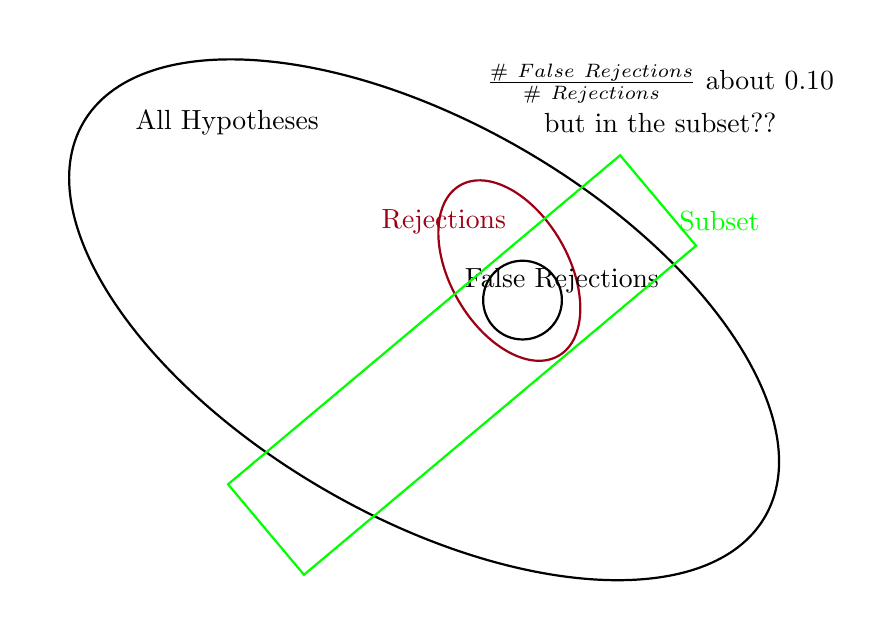
\begin{tikzpicture}[scale=2.5]
\draw[rotate=60,thick] (0,0) ellipse (1cm and 2cm);
\path (-1,1) node {All Hypotheses};
\draw[rotate=30,thick, redUnipd] (.5cm,0) ellipse (.3cm and .5cm);
\path[redUnipd] (.1,.5) node {Rejections};
\pause
\draw[rotate=00,thick, black] (.5cm,.1) ellipse (.2cm and .2cm);
\path[black] (.7,.2) node {False Rejections};
\path[black] (1.2,1.2) node {$\frac{\#\ False\ Rejections}{\#\ Rejections}$ about $0.10$};
\pause
\path[black] (1.2,1) node {but in the subset??};
\draw [rotate=40,green,thick] (-1.3, -.6) rectangle (1.3,0);
\path [green] (1.5,.5) node {Subset};
\end{tikzpicture}
\end{frame}




\bfr{Relationships between FWER and FDR}
  \bb{Dominance}
    \[ \mathrm{P}(V > 0) = \mathrm{E}(\boldsymbol{1}\{V > 0\}) \geq \mathrm{E}(\mathrm{FDP}) \]
    Consequence: Control of FWER implies control of FDR
  \eb
  \bb{Complete null hypothesis}
    If all hypotheses true, $\mathrm{FDP} = \boldsymbol{1}\{V > 0\}$
    \\ Consequence: If all hypotheses true, FDR $=$ FWER
  \eb
  \bb{Single hypothesis}
    If only one hypothesis, $\mathrm{FDP} = \boldsymbol{1}\{V > 0\}$
    \\ Consequence: If only one hypothesis, FDR $=$ FWER $=$ Type I error
  \eb
\end{frame}


\bfr{FWER vs.\ FDR: scaling}
  \bb{Scaling}
    As the size $m$ of the problem grows \\(complete null not true)
  \eb
  \bb{FWER}
    \bi
      \item Number of rejections remains limited
      \item Number of errors remains limited
    \ei
  \eb
  \bb{FDR}
    \bi
      \item Number of rejections grows with $m$
      \item Number of errors grows with $m$
    \ei
  \eb
\end{frame}


\bfr{When to use FDR}
%   \bb{Use FDR especially}
    \bi
      \item If collection of rejections important
      \item If validation experiments follow
      \item If hypotheses are exchangeable
      \item If power is an issue
    \ei
%   \eb
\end{frame}


\subsection{}
\bfr{Take-home message}
\bi 
\item molteplicity control is mandatory in Clinical Trials 
\item FWER: controlling the probability of at least one error
\item FDR:  controlling the  proportion of false rejection (on average)
\item FWER is 
\bi
\item a stronger control
\item usually preferible in Clinical Trials
\item more flexible
\ei
\item FWER and FDR  easy in {\tt R}
\item excellent tutorial: Goeman \& Solari (2014) \footnote{
JJ Goeman, A Solari (2014) Tutorial in biostatistics: multiple hypothesis testing in genomics. Statistics in medicine, Volume 33, Issue 11}
\ei
\end{frame}



\end{document}


